%https://books.google.cz/books?id=DiFMPmXSsLUC&pg=SA6-PA15&lpg=SA6-PA15&dq=Varshni+1967&source=bl&ots=hBJXnBqrHH&sig=WuCbtLj6FUIWMr09BP1LkBR-2cc&hl=cs&sa=X&ved=0ahUKEwi5mPz5lL_ZAhUGEVAKHRiaAOIQ6AEIXDAH#v=onepage&q=Varshni%201967&f=false

\chapter{Excitonic structure and pumping power dependent emission blue-shift of type-II quantum dots}
\label{chap:SciRep}


Semiconductor quantum dots (QDs) are one of the most promising candidate systems for the realization of quantum cryptography protocols~\citep{Muller2014,Strauf2007} or quantum gates~\citep{Stevenson2006,Rodt} in the information technologies. Most of the interest in the literature is focused on type-I QDs with both electron and hole states confined in the QD body. 
The spatial separation of the quasiparticle wavefunctions in type-II QDs leads to smaller overlap of the wavefunctions resulting in reduced emission intensity and recombination rate~\citep{Klenovsky10,KleJOPCS,Hsu,Nishikawa2012}. Moreover, a large blue-shift of emission energy with increasing laser pumping has been observed~\citep{Jin,UlloaHomogSRL}. The carrier separation in type-II confined systems has several advantages compared to the type-I. In particular, a naturally small fine-structure splitting (FSS)~\citep{Krapek2015} and molecular-like states~\citep{Klenovsky10,KleJOPCS,KrapekNottingham} were predicted. As a result, type-II QDs can be used in quantum information technology without the need for post-processing of the quantum states. 

There has been only a small number of studies of the excitonic structure of type-II QDs~\citep{Matsuda2007,Miloszewski2014} due to their inhomogeneous broadening of the spectral bands. Hence, in this chapter we investigate the multi-particle states by experimental observation of the recombination using intensity and polarization resolved photoluminiscence (PL) measurements of InAs/GaAsSb/GaAs QDs. Our experiment is supported by theoretical description by a Full Configuration Interaction (CI) developed by the supervisor~\citep{Klenovsky2017}. Finally, we have simulated the experimentally observed blue-shift of the emission of these QDs using a semi-self-consistent CI algorithm~\citep{Klenovsky2017}.

\medskip
For the theoretical description and the experimental testing we have chosen GaAsSb capped InAs QDs in GaAs matrix. This system is favoured because it allows continuous change of type confinement by varying Sb content in GaAsSb capping layer~\citep{Klenovsky10}.

\medskip
In this chapter we present results of theoretical calculations of the multi-particle structure of our system performed by the supervisor, followed by experimental verification of that done by the author of this thesis. Note, that we show here the former mainly as a guide to the experiments.
\newpage 




\section{Multi-excitonic structure calculation} \label{sec:scirep_theory}
The supervisor calculated the multi-excitonic structure of the studied QDs by the CI method. The single-particle basis states were obtained from the Nextnano++ simulation package~\citep{next} using the envelope function approximation based on the eight-band $\mathbf{k \cdot p}$ method. The In distribution in a simulated lens shape InAs QD with height of 4~nm and basis diameter of 16~nm was either constant at 0.6, or trumpet-like. The thickness $d$ and Sb composition of the CL were varied during calculations. 
%
\begin{figure}
	\centering
	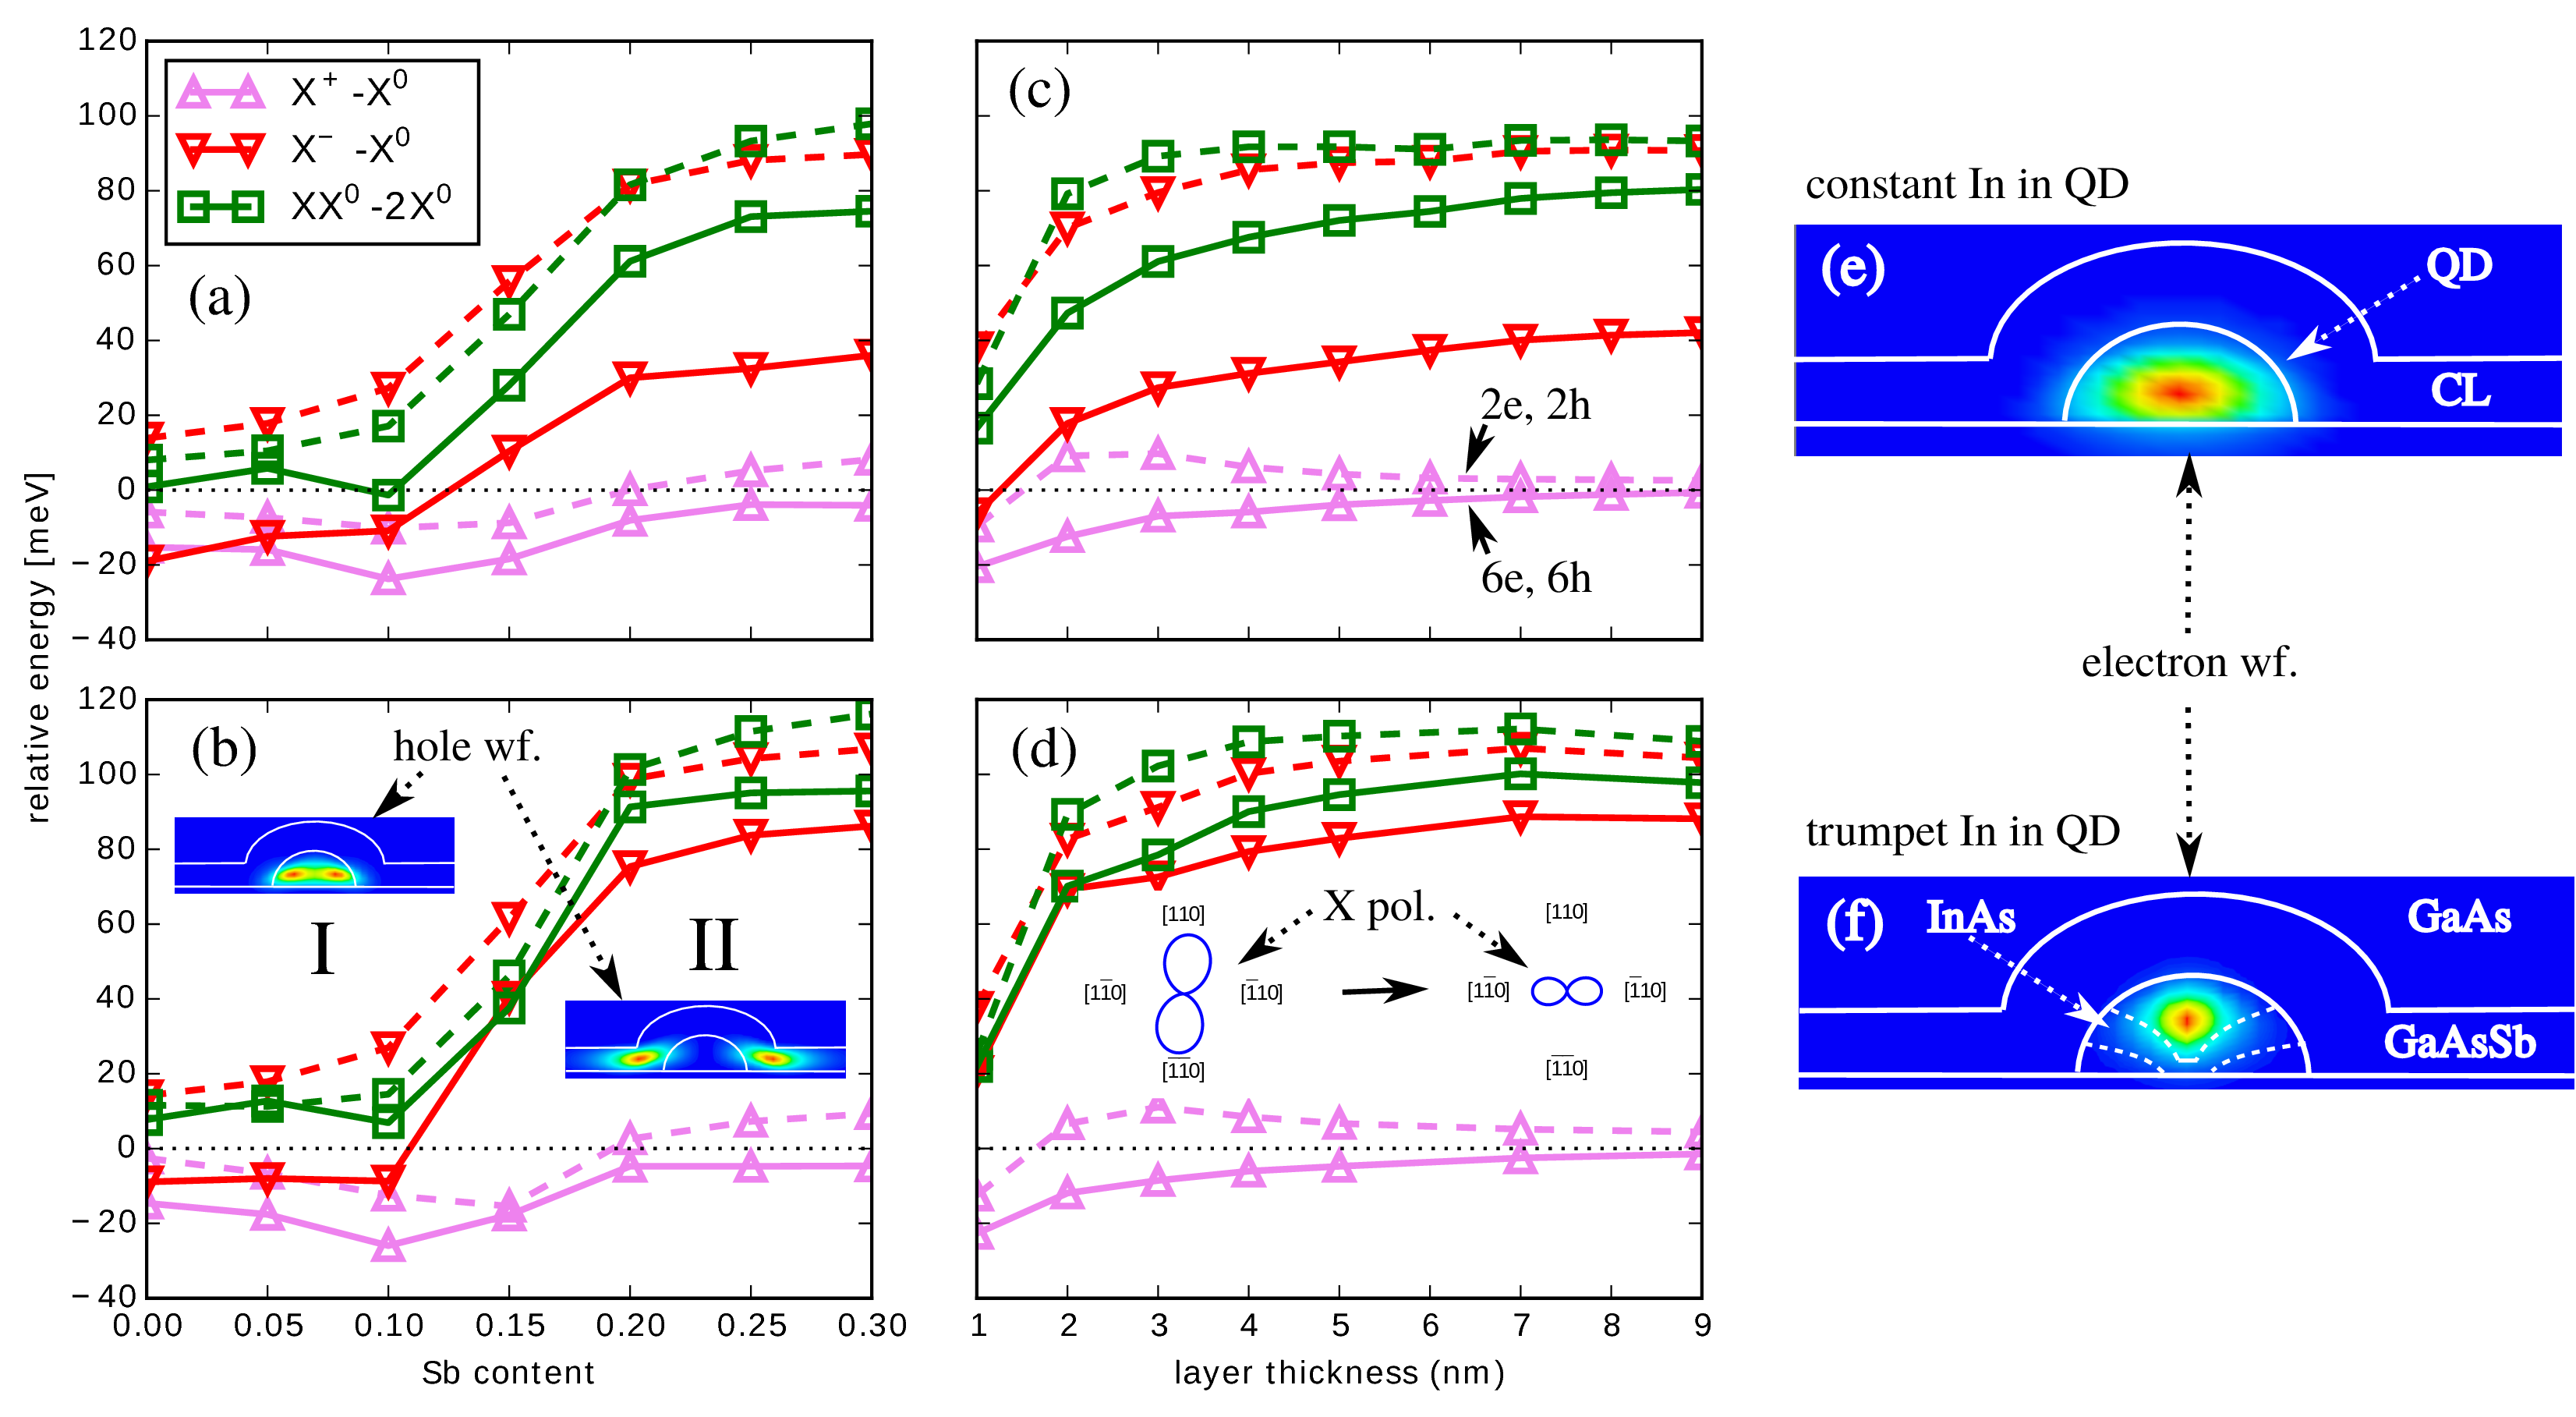
\includegraphics[width=1\linewidth]{/Sci_rep/article/theory}
	\caption{Energies of the complexes $X^+$, $X^-$, and $XX^0$ with respect to that of $X^0$ as functions of (a, b) Sb content for a constant and trumpet In composition in QD with CL thickness $d=5~\mathrm{nm}$, respectively, and (c, d) $d$ for fixed Sb content of 0.24 in the same QDs. The dashed lines are connected to calculations with 2 electron and 2 hole single-particle basis states while the full lines with 6~by~6 basis. In insets of panel~(b) are $(1\overline{1}0)$~plane cuts of the hole probability densities, and labels I and II represent the type of confinement. The inset of (d) illustrates the polarization of the emission of $X^0$ for thin and thick CL. Panels (e) and (f) show simulated structures and probability density of the electron wavefunction in QD for constant In content of 0.6 and trumpet In distribution, respectively.}
	\label{fig:Sci_rep_theory}
\end{figure}
%

In Fig.~\ref{fig:Sci_rep_theory}~(a) and (b) we show the calculated Sb content dependencies of the energy differences of $X^+$, $X^-$ and $XX^0$ from $X^0$ for QD with constant In content [panel (a)] and trumpet In composition~\cite{Migliorato} [panel (b)], respectively. It can be seen that transition associated with $X^-$ and $XX^0$ becomes significantly anti-binding in type-II confined structures where holes are located in CL whereas electrons in QD body (see the inset of Fig.~\ref{fig:Sci_rep_theory}~(b) for the hole, and panels (e) and (f) for the electron wavefunctions). However, if the CL is too thin the energy of holes is too large for localization of the hole ground state in the CL and the system is type-I with increasing value of binding energy of complexes that is demonstrated for heterostructure with varying $d$ of CL for a fixed Sb content of 0.24 in Fig.~\ref{fig:Sci_rep_theory}~(c) and (d). Moreover, the increase of $d$ leads to a change in the vertical position of the hole wavefunction from the base of QD to above its apex. This is connected with a change in the orientation of the emission polarization and allows the determination of the vertical position of the hole from polarization resolved PL measurements, see Ref.~\citep{Klenovsky2016}. 

The binding energies of $XX^0$ and $X^-$ in type-II are, depending on the calculated dependencies and In distribution, in the range of 60--120~meV and 20--90~meV. On the other hand, in all our simulations $X^+$ remains rather anti-binding, more precisely its binding energy is between -20 and 5~meV. Detailed information about CI method and more detailed analysis of the results can be found in Ref.~\citep{Klenovsky2017}.


\section{InAs/GaAsSb/GaAs QD samples}
%For the theoretical description and the experimental testing have chosen GaAsSb capped InAs QDs in GaAs matrix. This system is favoured because it allows continuous change of type confinement by varying Sb content in GaAsSb capping layer~\citep{Klenovsky10} as can be seen in Fig.~\ref{fig:Sci_rep_theory}(a) and (b), where are the Sb content dependencies of the energy differences of $X^+$, $X^-$ and $XX^0$ from $X^0$ calculated by the supervisor using CI method, for details see Ref.~\citep{Klenovsky2017} or Sec.~\ref{Sec:CI}.

Structures for PL measurements were prepared by AIXTRON~200 on a non-rotating graphite susceptor on GaAs(100) substrate using a low pressure (7~kPa) metal-organic vapour phase epitaxy (MOVPE) in Stranski-Krastanov mode growth at the Institute of Physics of the Czech Academy of Sciences (FZU). First, the temperature was set to 650~$^\circ$C for the growth of the first GaAs buffer layer, then that was reduced to 510~$^\circ$C for the growth of the rest of the structure: (i) 10~nm thick GaAs buffer layer, (ii) 2 monolayers (MLs) of InAs for the growtn of QDs, (iii) 5~nm of GaAsSb capping layer (CL) and (iv) 100~nm GaAs finishing layer. Information about used precursors and growth rate can be found in Ref.~\citep{Klenovsky2016}.

For comparison with the measured phenomena of type-II QDs, we examined also type-I InAs/GaAs(001) QDs with a stack of 3 layers of InAs dots grown above each other by MOVPE in Stranski-Krastanov mode. For more information see Ref.~\citep{HumPhysE}.

\section{Photoluminescence setup}
%
\begin{figure}
	\centering
	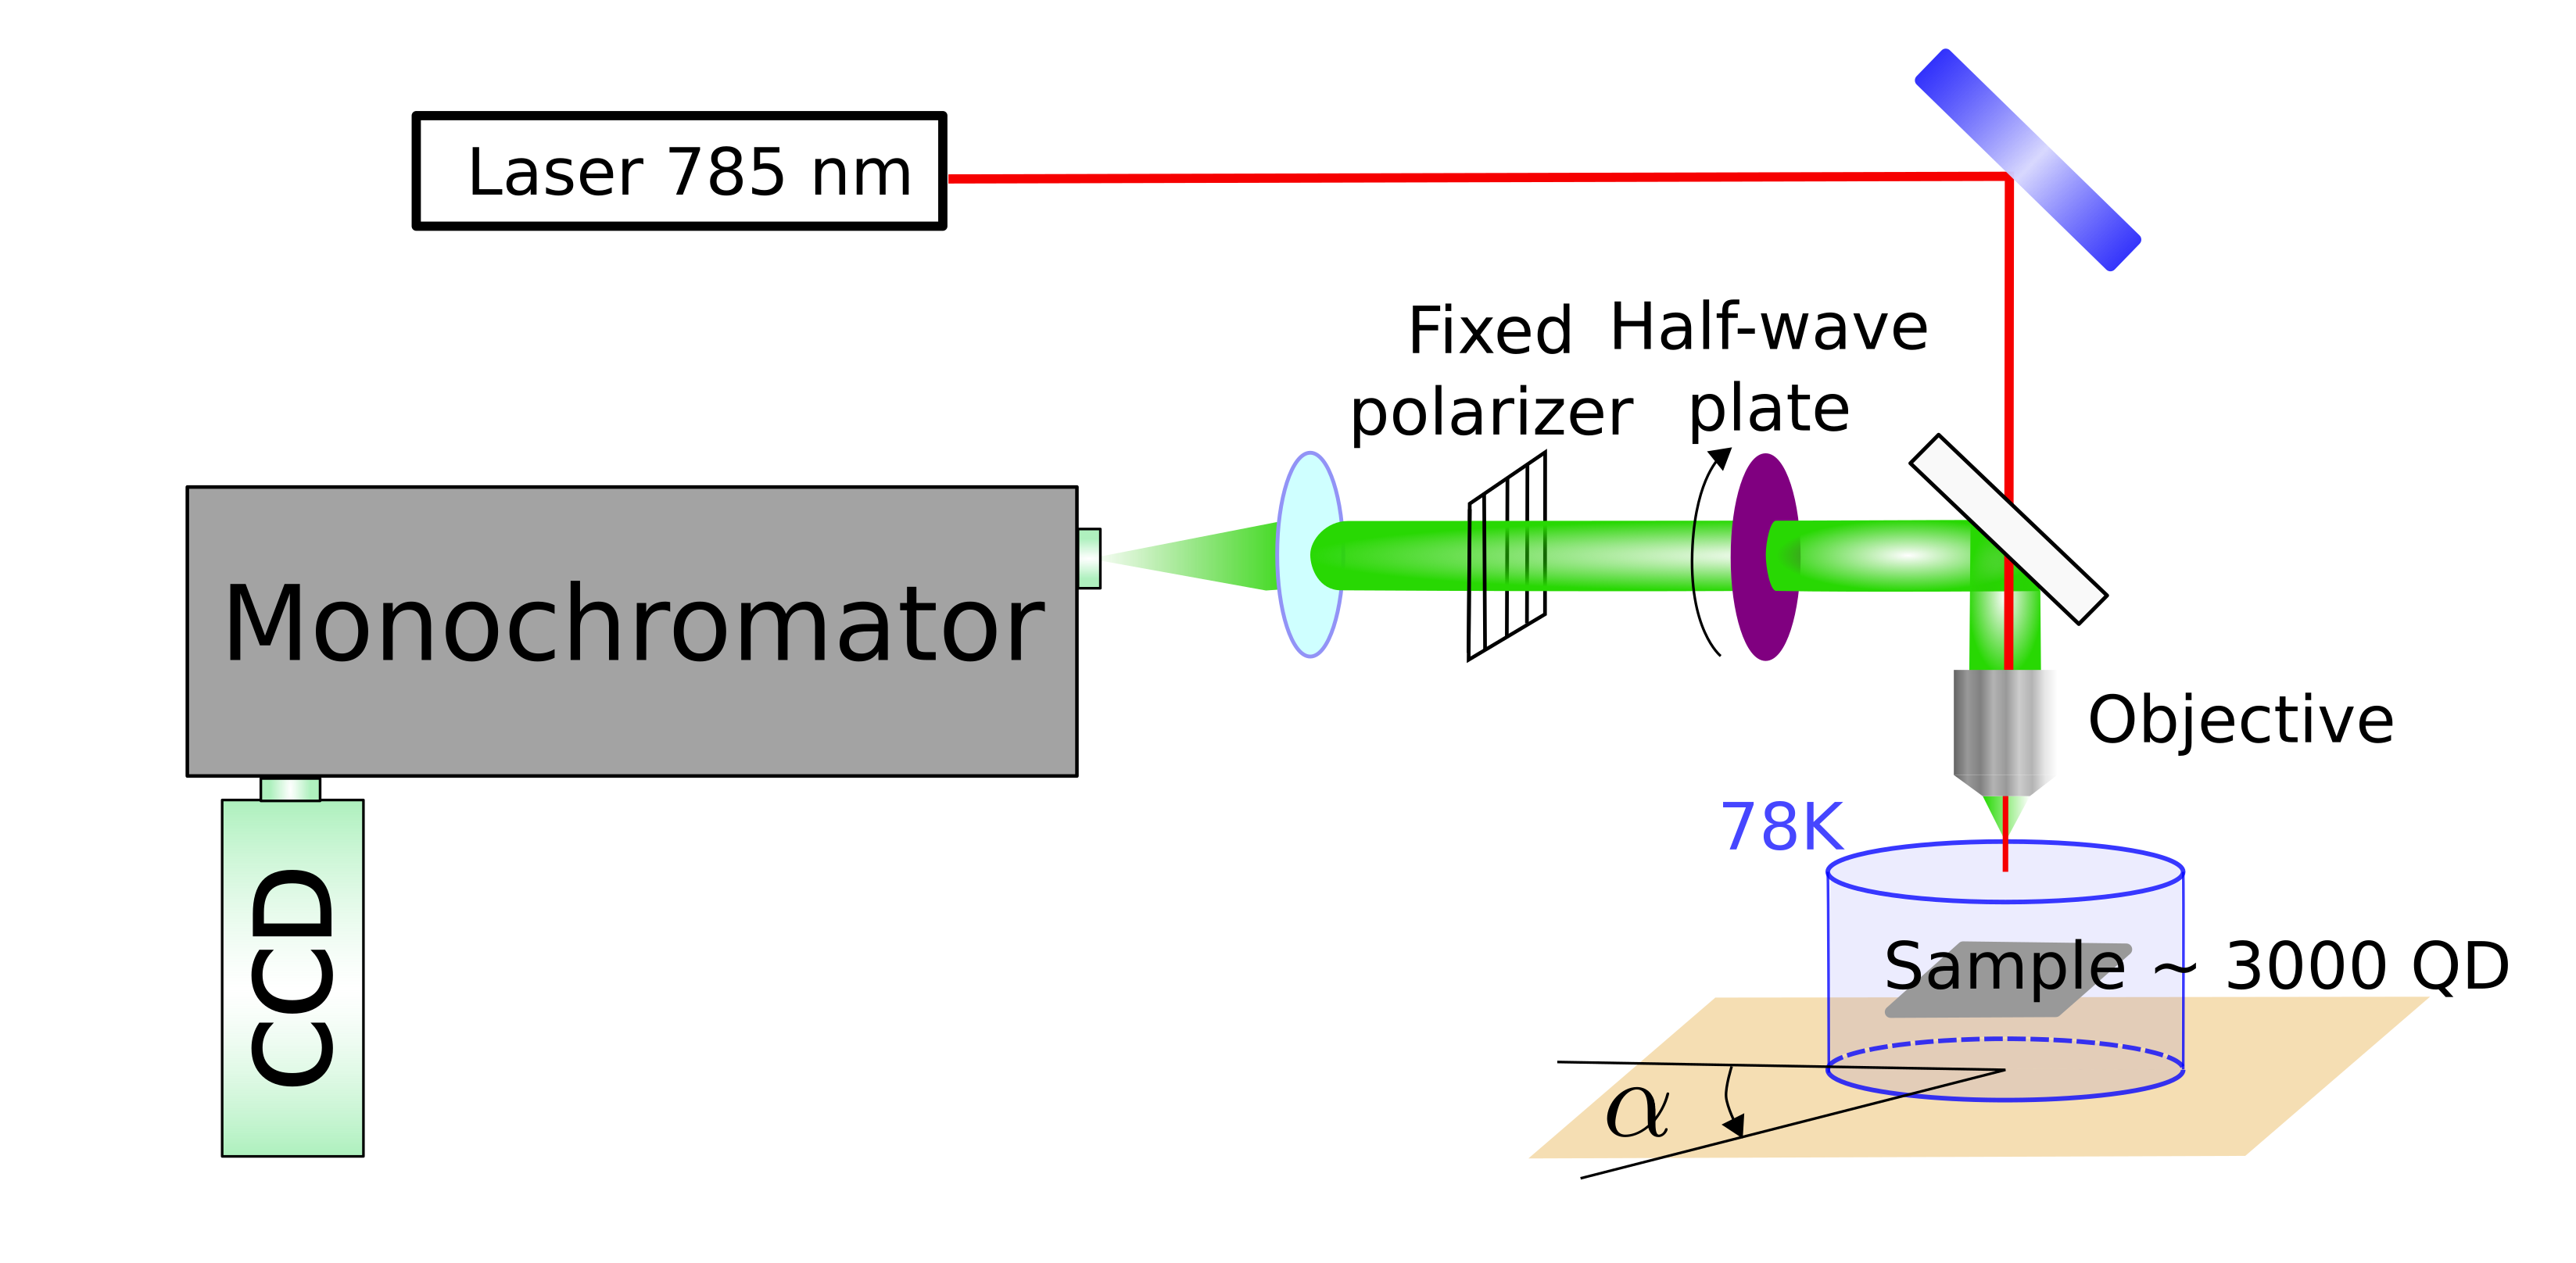
\includegraphics[width=0.9\linewidth]{/Sci_rep/article/setup_scirep}
	\caption{A sketch of the PL setup.}
	\label{fig:}
\end{figure}
The PL measurements were performed using the NT-MDT Ntegra-Spectra spectrometer. The samples were cooled to liquid nitrogen temperature and pumped by a solid-state laser with the emission wavelength of 785~nm. The maximum laser power on the surface was 5~mW focused by lens on 150~$\mu\mathrm{m}^2$ area and laser intensity was varied using a neutral density (ND) filter. 

%
The polarization of the emission spectrum was analyzed by a rotating achromatic half-wave retarder with the maximal transmission at 1300~nm followed by a fixed Glan-Taylor linear polarizer. The PL signal was dispersed by a 150~grooves/mm ruled grating and detected by the InGaAs line-CCD camera, cooled to minus 90~$^\circ$C to reduce thermal noise. In every experiment, PL signal was collected from a large number of QDs ($\sim$3000). Because the transmission of the setup depends on the photon energy, we have eliminated this effect by calibration to blackbody emission. 


The efficiency of the InGaAs CCD camera and emission spectrum of calibration source are depicted in Fig.~\ref{fig:calib_scirep}.
\begin{figure}
	\centering
	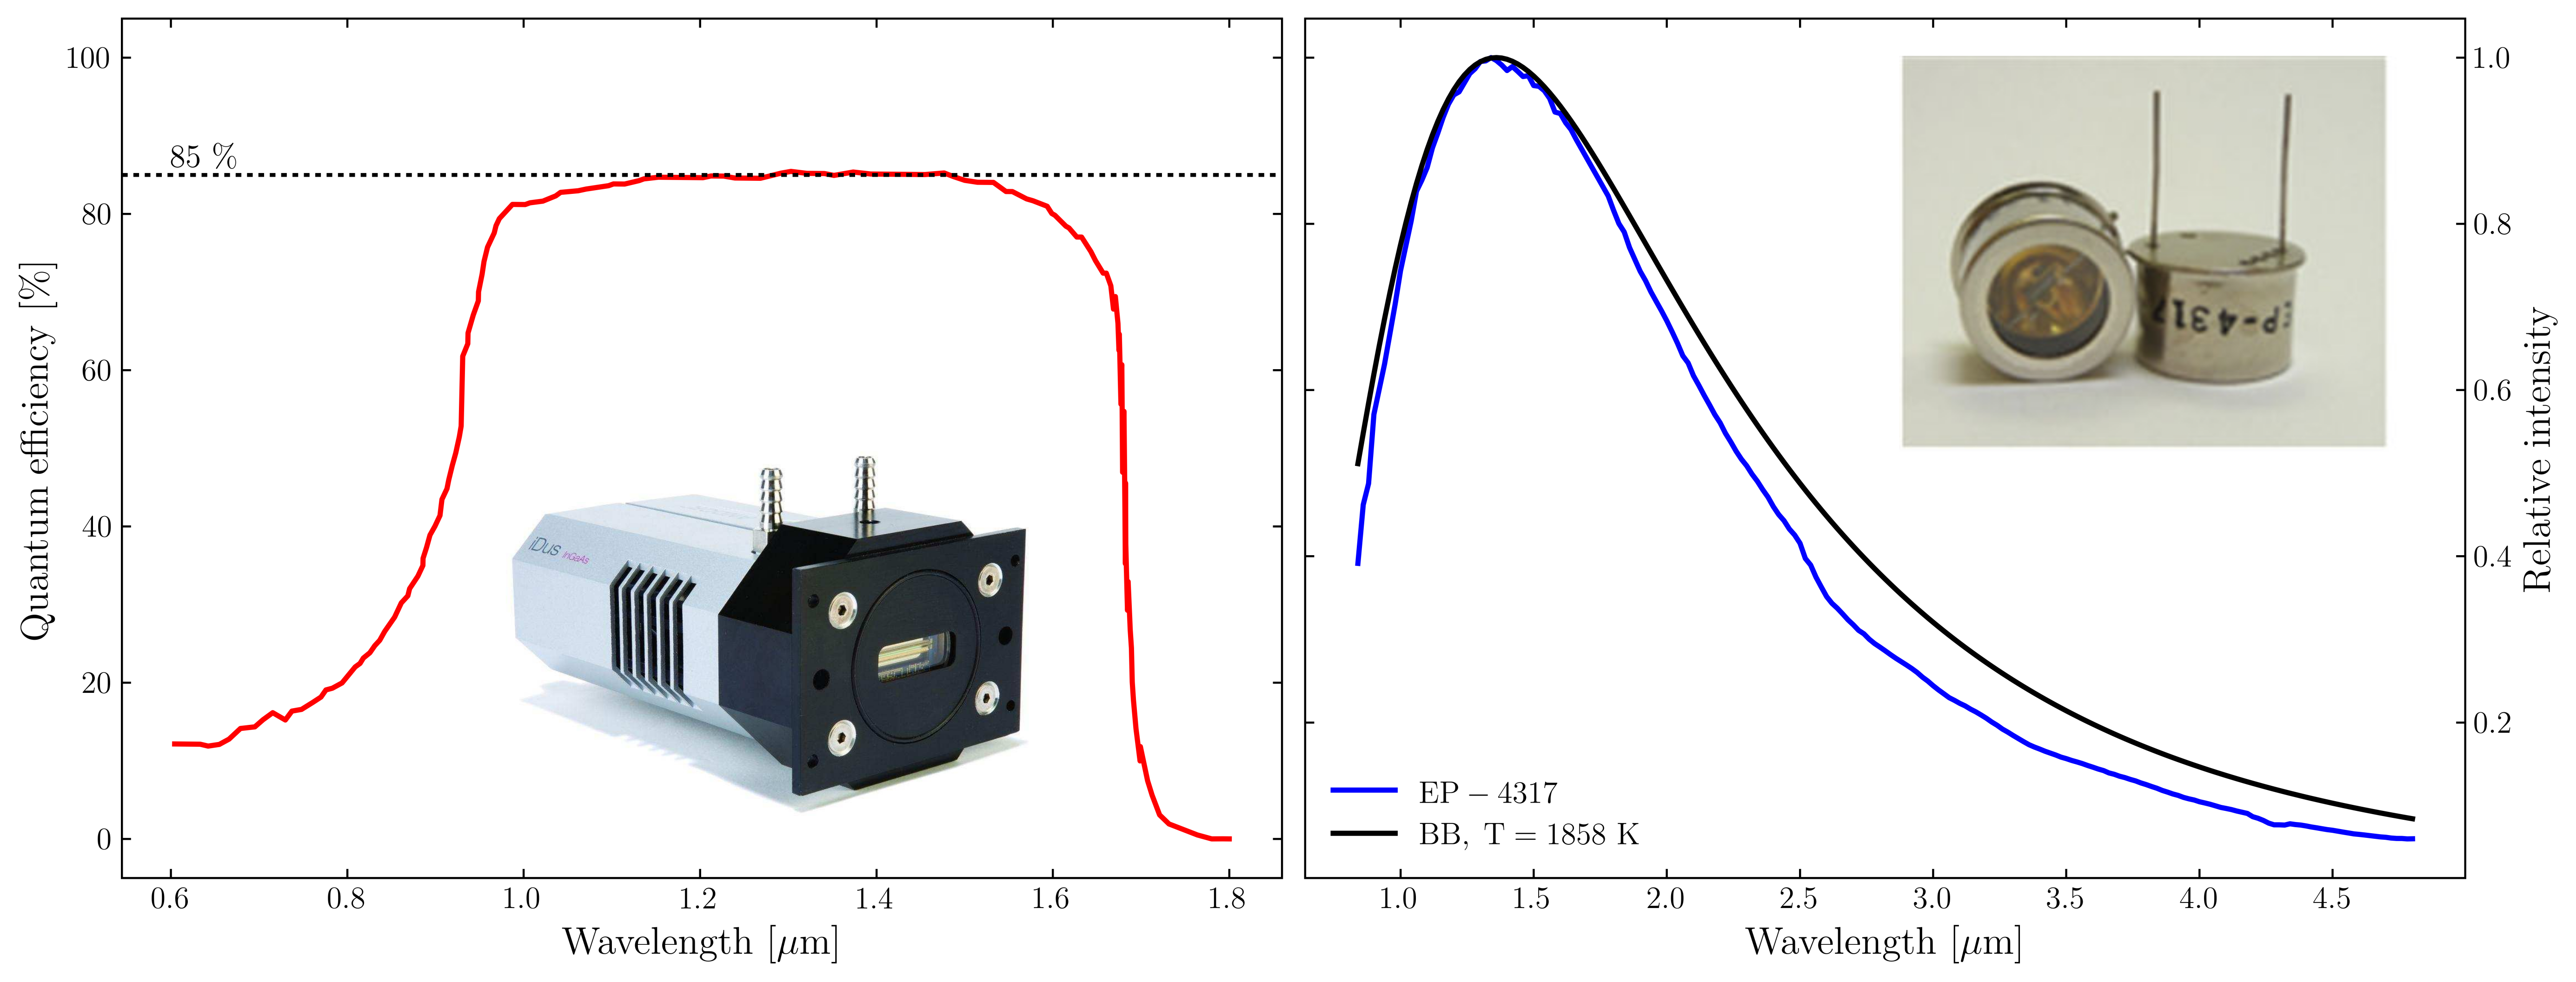
\includegraphics[width=0.9\linewidth]{/Sci_rep/article/ANDOR}
	\caption{Quantum efficiency of used \textit{ANDOR DU490A} camera at $T=20~^\circ$C, taken from Ref.~\citep{manual_andor}, and emission spectrum of a calibration source \textit{EP-4317} from Ref.~\citep{manual_BB} with its emission described by the Planck's law~\citep{Planck_law} characterized by temperature $T=1858~^\circ$C.}
	\label{fig:calib_scirep}
\end{figure}

\section{Photoluminescence measurements}
We show our experimental results for one sample with type-II QDs in Fig.~\ref{fig:sci_rep_typeII}. We measured PL spectra for a set of values of the laser pumping power $P$ and for each of these values also the polarization anisotropy defined by a degree of polarization $C(\alpha)$
\begin{equation}
C(\alpha)=\frac{F(\alpha)-F_\mathrm{min}}{F_\mathrm{max}+F_\mathrm{min}},
\end{equation}
where $\alpha$ is the angle corresponding to the crystallographic direction in the plane of the sample, $F_\mathrm{mix}$ and $F_\mathrm{max}$ are extremal values of the oscillator strength of the interband optical transition~$F$, respectively. The maximum of the degree of polarization $C_\mathrm{max}$ occurs in a direction given by the angle $\alpha_\mathrm{max}$. The spectra were fitted by a sum of 4~Gaussian functions and appropriate recombination channels were assigned, see Fig.~\ref{fig:sci_rep_typeII}(a). The assignment was based on (i) the exponent $a$ of $F\propto P^a$, see Fig.~\ref{fig:sci_rep_typeII}(b), (ii) the azimuth $\alpha_\mathrm{max}$, see the polar graphs at the bottom of Fig.~\ref{fig:sci_rep_typeII}, (iii) and comparison with the theoretical calculations summarized in Sec.~\ref{sec:scirep_theory}. The type of the confinement was determined by the observation of the blue-shift of the normalized PL spectra with increasing $P$ for type-II, or its absence for type-I, see panel~(a).

We clearly identified the recombination of $X^0$ with emission energy of 980~meV, $X^-$ and $XX^0$ in our PL spectra. The measured energy separation of these complexes from $X^0$ are $X^- - X^0=76$~meV and $XX^0-2X^0=162$~meV, i.~e. considerably shifted to higher energies as predicted by the theory, see Fig.~\ref{fig:Sci_rep_theory}. As expected, the band $X^+$ cannot be distinguished from $X^0$ in our PL measurements since the energy separation $X^+-X^0$ is much smaller than the inhomogeneous spectral broadening of the emission bands from GaAsSb capped InAs QDs.%
\begin{figure}
	\centering
	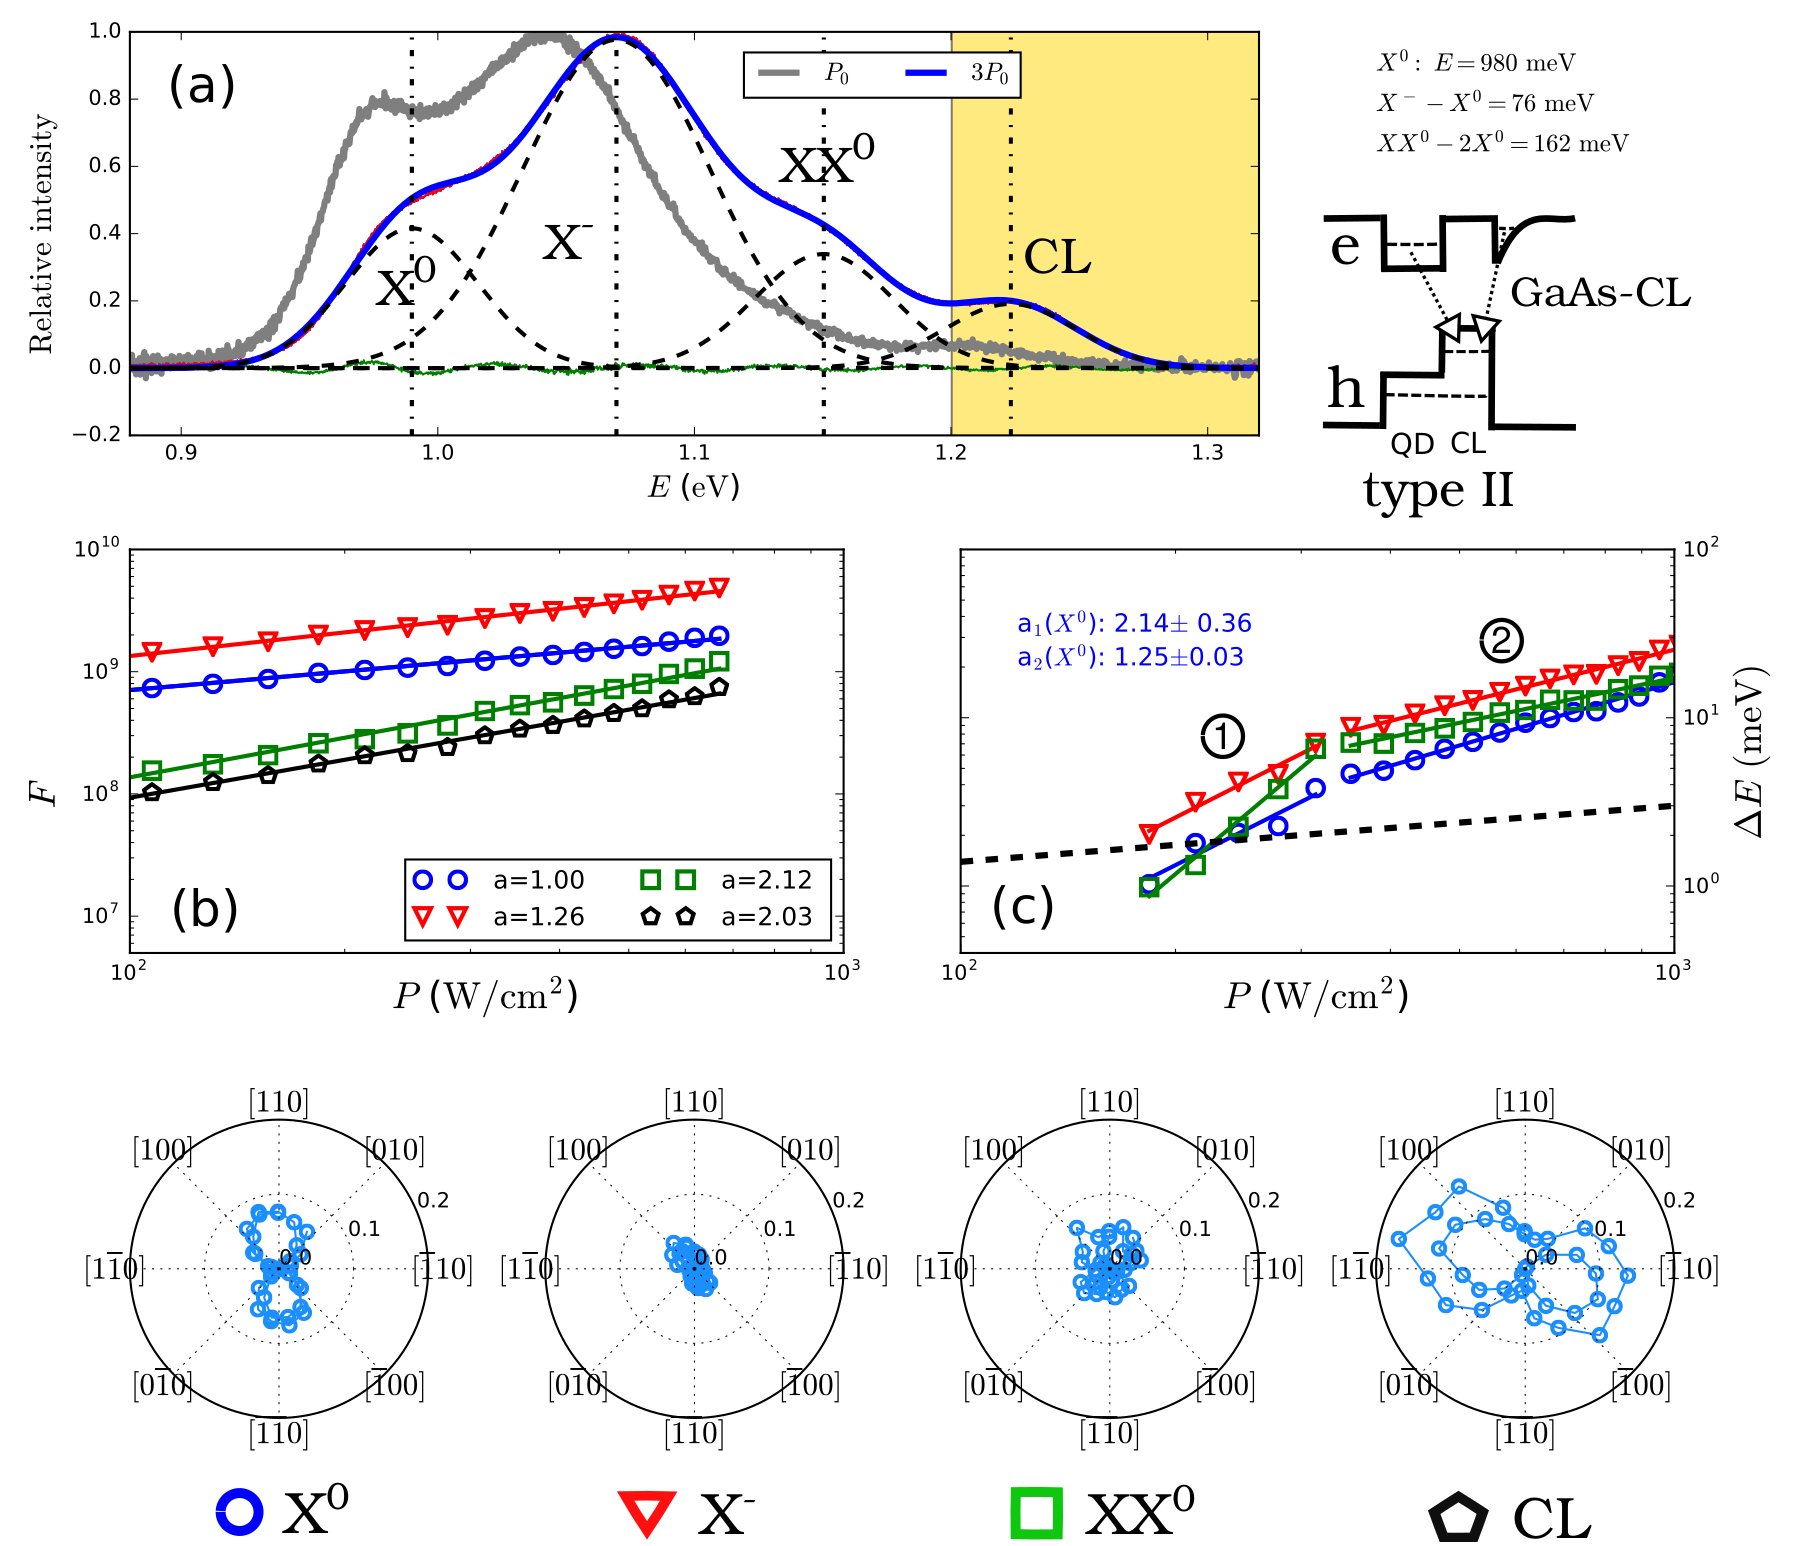
\includegraphics[width=0.9\linewidth]{/Sci_rep/article/type2}
	\caption{(a) PL spectra of GaAsSb capped InAs type-II QDs measured for two pumping powers $P$ (grey for $P_0=1.7$~mW and blue curve for $3P_0=5$~mW). The fit by a sum of 4~Gaussian profiles is shown for the PL spectrum obtained under 5~mW excitation power and the individual bands corresponding to different multi-excitonic transitions are shown by dashed lines. The difference between measured data and their fits is represented by the green line. The vertical dotted lines indicate the energies of the bands for $3P_0$. The yellow shaded part of the graph corresponds to the recombination between bulk GaAs and CL. The inset near to the panel~(a) gives the spectral position of the complexes from QDs and schematic band diagram of the recombination processes (not in scale). In (b) we show $P$-dependence of the oscillator strength $F$ of the identified bands in log-log scale and their fits by linear lines for $X^0$ (blue circles), $X^-$ (red triangles), $XX^0$ (green squares), and that for the transition between bulk GaAs and CL (black pentagons). The slopes $a$ (i.e. exponents in the linear plots) of the fitted lines are given in the inset of panel (b), for clarity they were normalized so that $a=1$ for $X^0$. Panel (c) depicts the change of the emission energy $\Delta E$ with $P$ in log-log scale. Except of GaAs-CL transition which was omitted, the labels are the same as in (b) and the data were fitted by two linear functions in segments 1 and 2 (see text). The fitted slopes (i.~e. exponents of the dependencies) $a_1$ and $a_2$ for $X^0$ are given in the inset. The $\Delta E\sim P^{1/3}$ dependence of Ref.~\citep{Hatami1998} is shown by the dashed line. The polar graphs at the bottom show $C(\alpha)$ of individually identified bands.}
	\label{fig:sci_rep_typeII}
\end{figure}

The band with the largest emission energy $E$ of 1.21~eV [shaded part of Fig.~\ref{fig:sci_rep_typeII}(a)] is attributed to the recombination between electrons confined due to strain at the interface between bulk GaAs and the GaAsSb CL, and holes within the GaAsSb CL, see also inset Fig.~\ref{fig:sci_rep_typeII}. This transition is purely of type-II and exhibits a very large blue-shift with increasing $P$. A similar recombination pattern has been observed previously for InAsSb QDs~\cite{Mazur2012} and is also responsible for the no-phonon emission from SiGe/Si QDs~\cite{SiGeKlenovsky}. 

To identify the bands also the exponent $a$ of $F\propto P^a$ was used, see log-log scale Fig.~\ref{fig:sci_rep_typeII}(b). The value of $a$ corresponding to probability $\mathcal{P}(M)$ of the excitation of the complex $M$. The oscillator strength of $X^0$ is proportional to probability $\mathcal{P}(X^0)$, therefore $F(X^0)\sim \mathcal{P}$. The biexciton $XX^0$ can be seen as a system of two excitons with expected $\mathcal{P}(XX^0)=\mathcal{P}(X^0)\cdot \mathcal{P}(X^0)\sim \mathcal{P}^2$ behaviour. The trion state $X^-$ (the complex consists of two electrons and one hole) is more probable than $XX^0$ but less probable than $X^0$ because in order to excite $X^-$ we need to generate $X^0$ and an extra electron, hence we expected $1<a(X^-)<2$. Consistently with previous findings, we obtained $a$ from our experiments. Other values of $a$ were normalized to the $a$ of the lowest band in emission energy, hence $a=1.0$ for $X^0$. The other $a$'s are $1.26$ for $X^-$, 2.12 for $XX^0$ and 2.02 for the transition between bulk GaAs and CL, respectively.


In Fig.~\ref{fig:sci_rep_typeII}~(c) in log-log scale the energy shift $\Delta E$ of the PL bands with increasing $P$ defined by
\begin{equation}
\Delta E(P)= E(P) - E(P_\mathrm{min}),
\end{equation}
is shown, where $P_\mathrm{min}$ is the lowest value of $P$ used in the corresponding experiment. In addition to a considerable blue-shift of the bands, which is as large as 30~meV for our values of $P$, it can be seen that (i) $\Delta E$ is different for different $M$ and (ii) there is an edge in the power dependencies meaning that $\Delta E(P)$ 
does not follow the simple form of $\Delta E\sim P^a$ for all values of $P$ but that for each of the two segments 1 and 2 a different exponents $a_1=2.14\pm0.36$ and $a_2=1.25\pm0.03$, respectively, seem more appropriate. That effect, observed also elsewhere~\citep{Muller-Kirsch2001}, is significantly different from the $\Delta E\sim P^{1/3}$ dependency predicted in Ref.~\citep{Hatami1998}, which is displayed as a dashed line for comparison.
Moreover, there are differences between the values of the exponents for different complexes. We postpone the explanation of the pumping dependent blue-shift to Sec.~\ref{sec:scirep_pumpingmodel}.

The polar graphs at the bottom of Fig.~\ref{fig:sci_rep_typeII} show that radiation of the recombination of complexes $M$ from the dots is polarized along [110]~crystallographic direction, which means that holes are located in the CL close to the QD base~\citep{Klenovsky2015}. Sharing the same $\alpha_\mathrm{max}$ for all $M$s confirms the prediction that all complexes due of the studied ensemble PL are polarized along the same direction, see Ref.~\citep{Klenovsky2017}. Moreover, the measurement of $\alpha_\mathrm{max}$ allows us to clearly distinguish the GaAs-CL band from the recombinations originating from QD states owing to their perpendicular polarization~\citep{Alonso-Alvarez2011a}.

In Fig.~\ref{fig:scirep_typeIq} we present PL measurements of QDs with type-I confinement in the same manner as in Fig.~\ref{fig:sci_rep_typeII}. We again identify $X^0$, $X^-$, $XX^0$ and the GaAs-CL transition, respectively, with the similar positions of $M$s to type-II QDs. Exciton $X^0$ is positioned at 982~meV, and $X^-$ and $XX^0$ are shifted to higher energies of about 80~meV and 173~meV, respectively. Similarly, considerable increase of $X^--X^0$ and $XX^0-2X^0$ occurs due to the fact that even a rather small increase in CL thickness results in a large increase of binding energies, as can be seen in Fig.~\ref{fig:Sci_rep_theory}. 
%
\begin{figure}
	\centering
	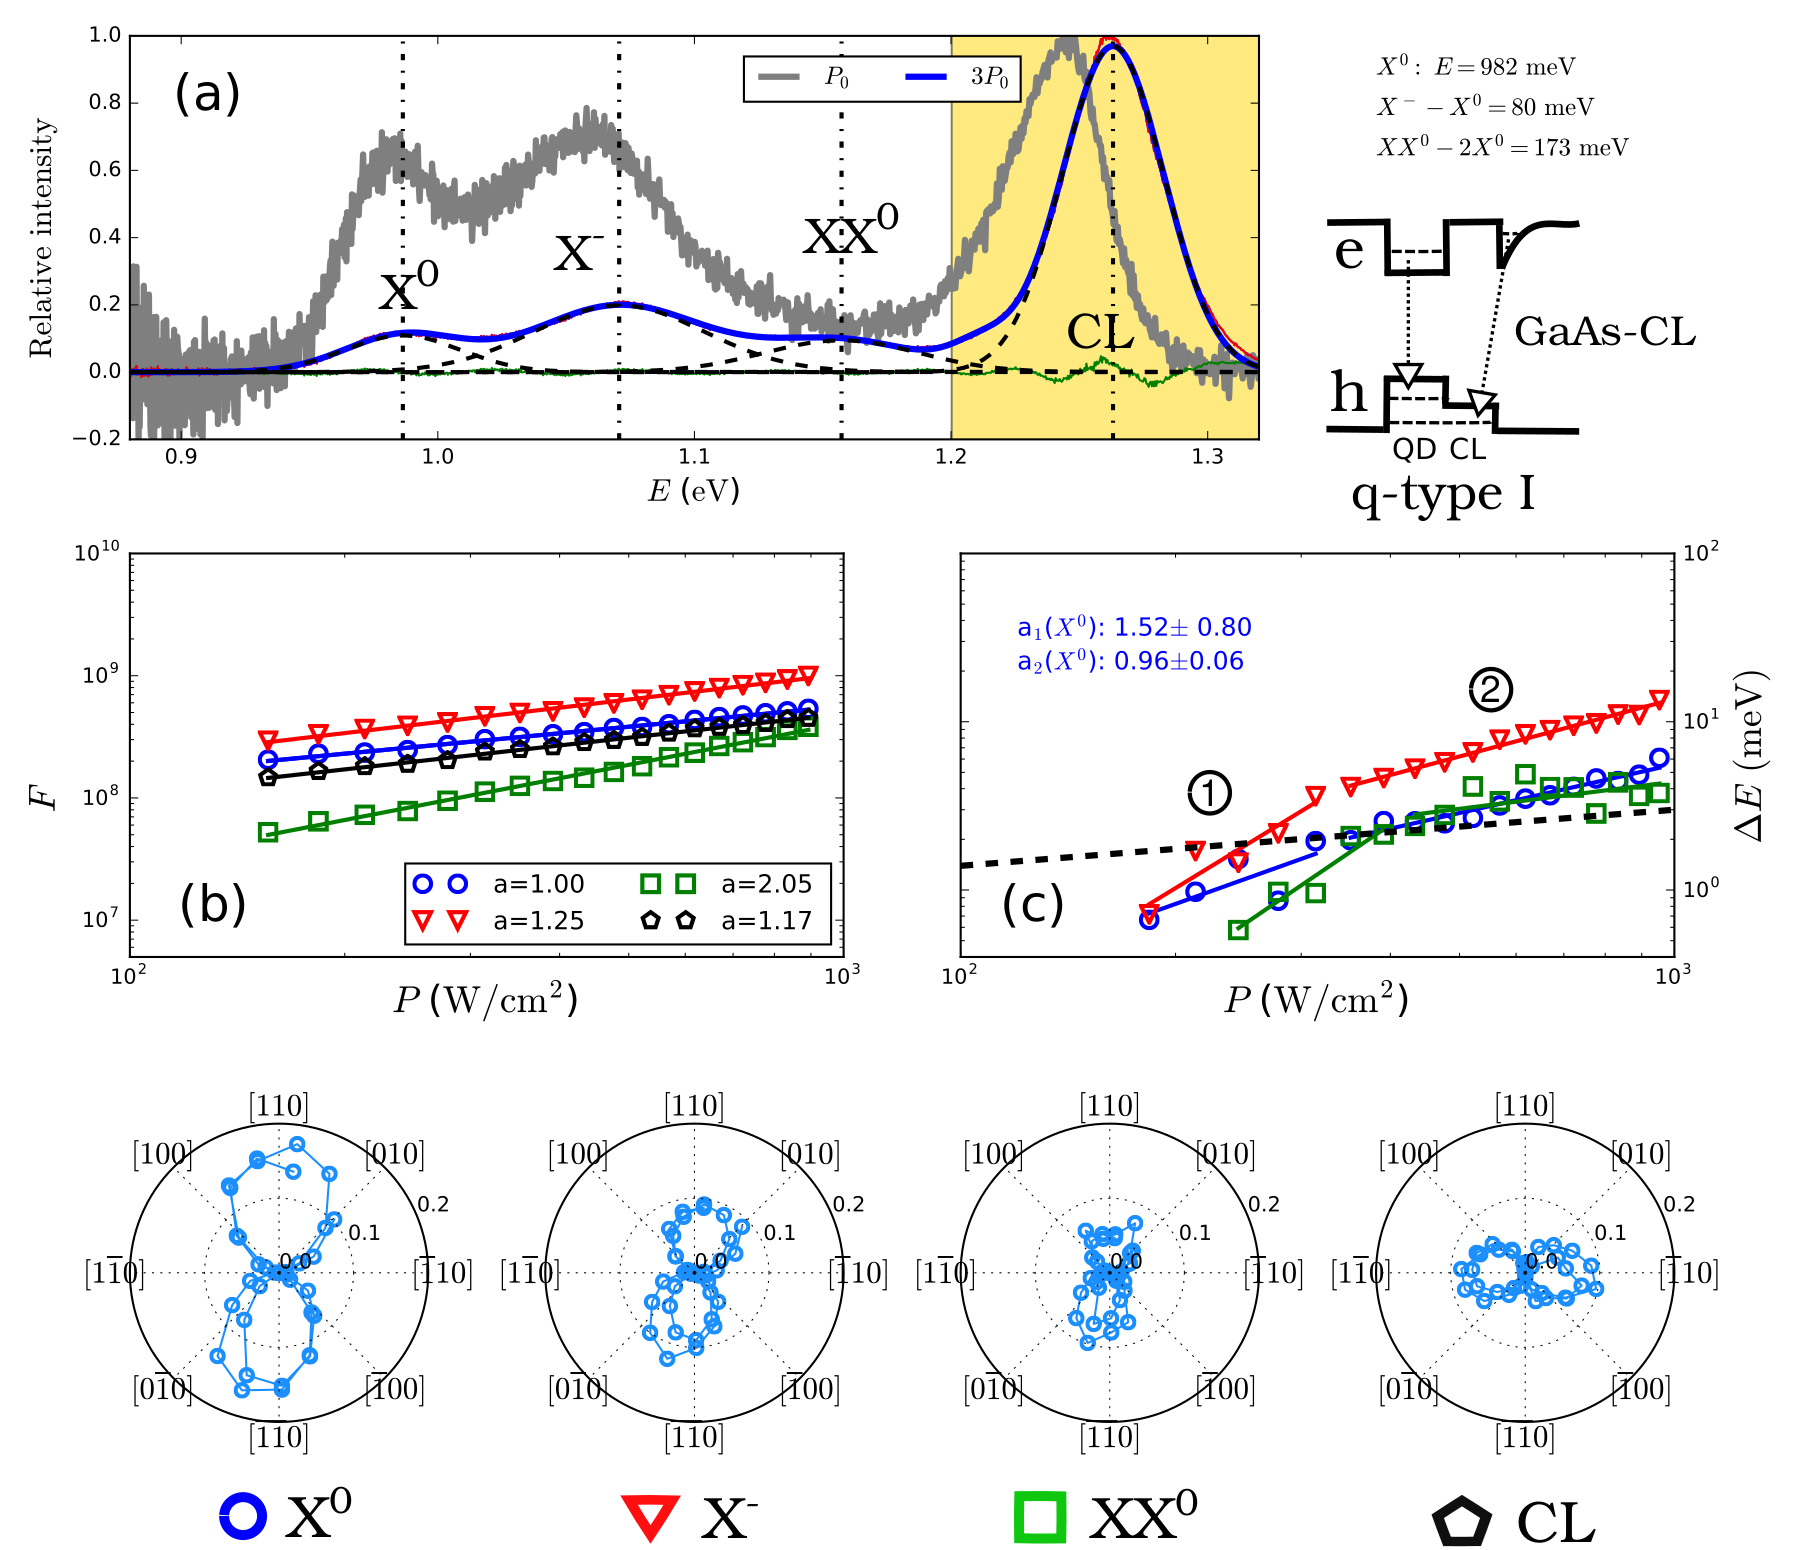
\includegraphics[width=0.9\linewidth]{/Sci_rep/article/typeI}
	\caption{PL spectra of GaAsSb capped InAs q-type-I QDs. The results are similarly commented as in Fig.~\ref{fig:sci_rep_typeII}.}
	\label{fig:scirep_typeIq}
\end{figure}
%
In fact, the type of confinement is not purely of type-I in GaAsSb capped InAs QDs for Sb contents different from zero, since even a slight increase of that lowers the confinement for holes in the CL with respect to GaAs~\cite{Klenovsky10}, see inset of Fig.~\ref{fig:scirep_typeIq}. Thus, the excited single-particle states tend to be partly localized in the CL, which results in a slight blue-shift of $X^0$ with increasing $P$ and also $a_1=1.52\pm0.80$ and $a_2=0.96\pm0.06$ are not equal to zero, see Fig.~\ref{fig:scirep_typeIq}~(c). We call this type of confinement \enquote{quasi-type-I} (q-type-I). For results of the true type-I confinement represented by InAs/GaAs QDs for which no blue-shift of $X^0$ with $P$ is observed and $a\approx0$ see Fig.~\ref{fig:671C}. We note that slightly larger values of $X^--X^0$ and $XX^0-2X^0$ for type-II and q-type-I in Figs.~\ref{fig:sci_rep_typeII} and~\ref{fig:scirep_typeIq}, respectively, compared to Fig.~\ref{fig:Sci_rep_theory} are probably due to the spatial inhomogeneity of the In distribution in the QDs, and of Sb in the CL, which were not considered in our theory. 

The polarization anisotropy of q-type-I QDs is again oriented along [110], see the bottom of Fig.~\ref{fig:scirep_typeIq}, and its degree is larger than for type-II in agreement with the trend for very thin CL discussed in Ref.~\citep{Klenovsky2017}. The GaAs-CL transition is again perpendicularly polarized compared to the emission of QD bands. Since the confinement for holes in the CL is larger for type I than for type II, the emission energy of GaAs-CL band is larger in type I. The energy of the GaAs-CL band also blue-shifts with pumping by a much larger amount than for the q-type-I QD bands and, thus, this structure represents a coexistence of type-I and type-II confinement~\cite{Ji2015}.


The pumping power dependence of PL from type-I InAs/GaAs QDs is shown in Fig.~\ref{fig:671C}. Using oscillator strength dependencies on $P$ we identify  $X^0$ and $XX^0$ optical transitions with appropriate slopes $a=1$ and $a=2.13$, respectively, with emission anisotropy along [110] crystallographic direction observing before in, e.~g.,~\citep{HumPhysE}. Note particularly that the energy of $X^0$ does not change with $P$, i.~e. $\Delta E\approx 0$. On the other hand, large blue-shift of $XX^0$ with $P$ is due to the structure of the sample. It is a stack of 3 layers of InAs QDs grown above each other. Due to that $XX^0$ in Fig.~\ref{fig:671C} originates in transitions when the quasi-particles are located in different QDs of the multilayer and are thus of type-II displaying considerable blue-shift with $P$. We note that biexcitons originating in transitions from one QD cannot be resolved by our PL measurements.
%
\begin{figure}
	\centering
	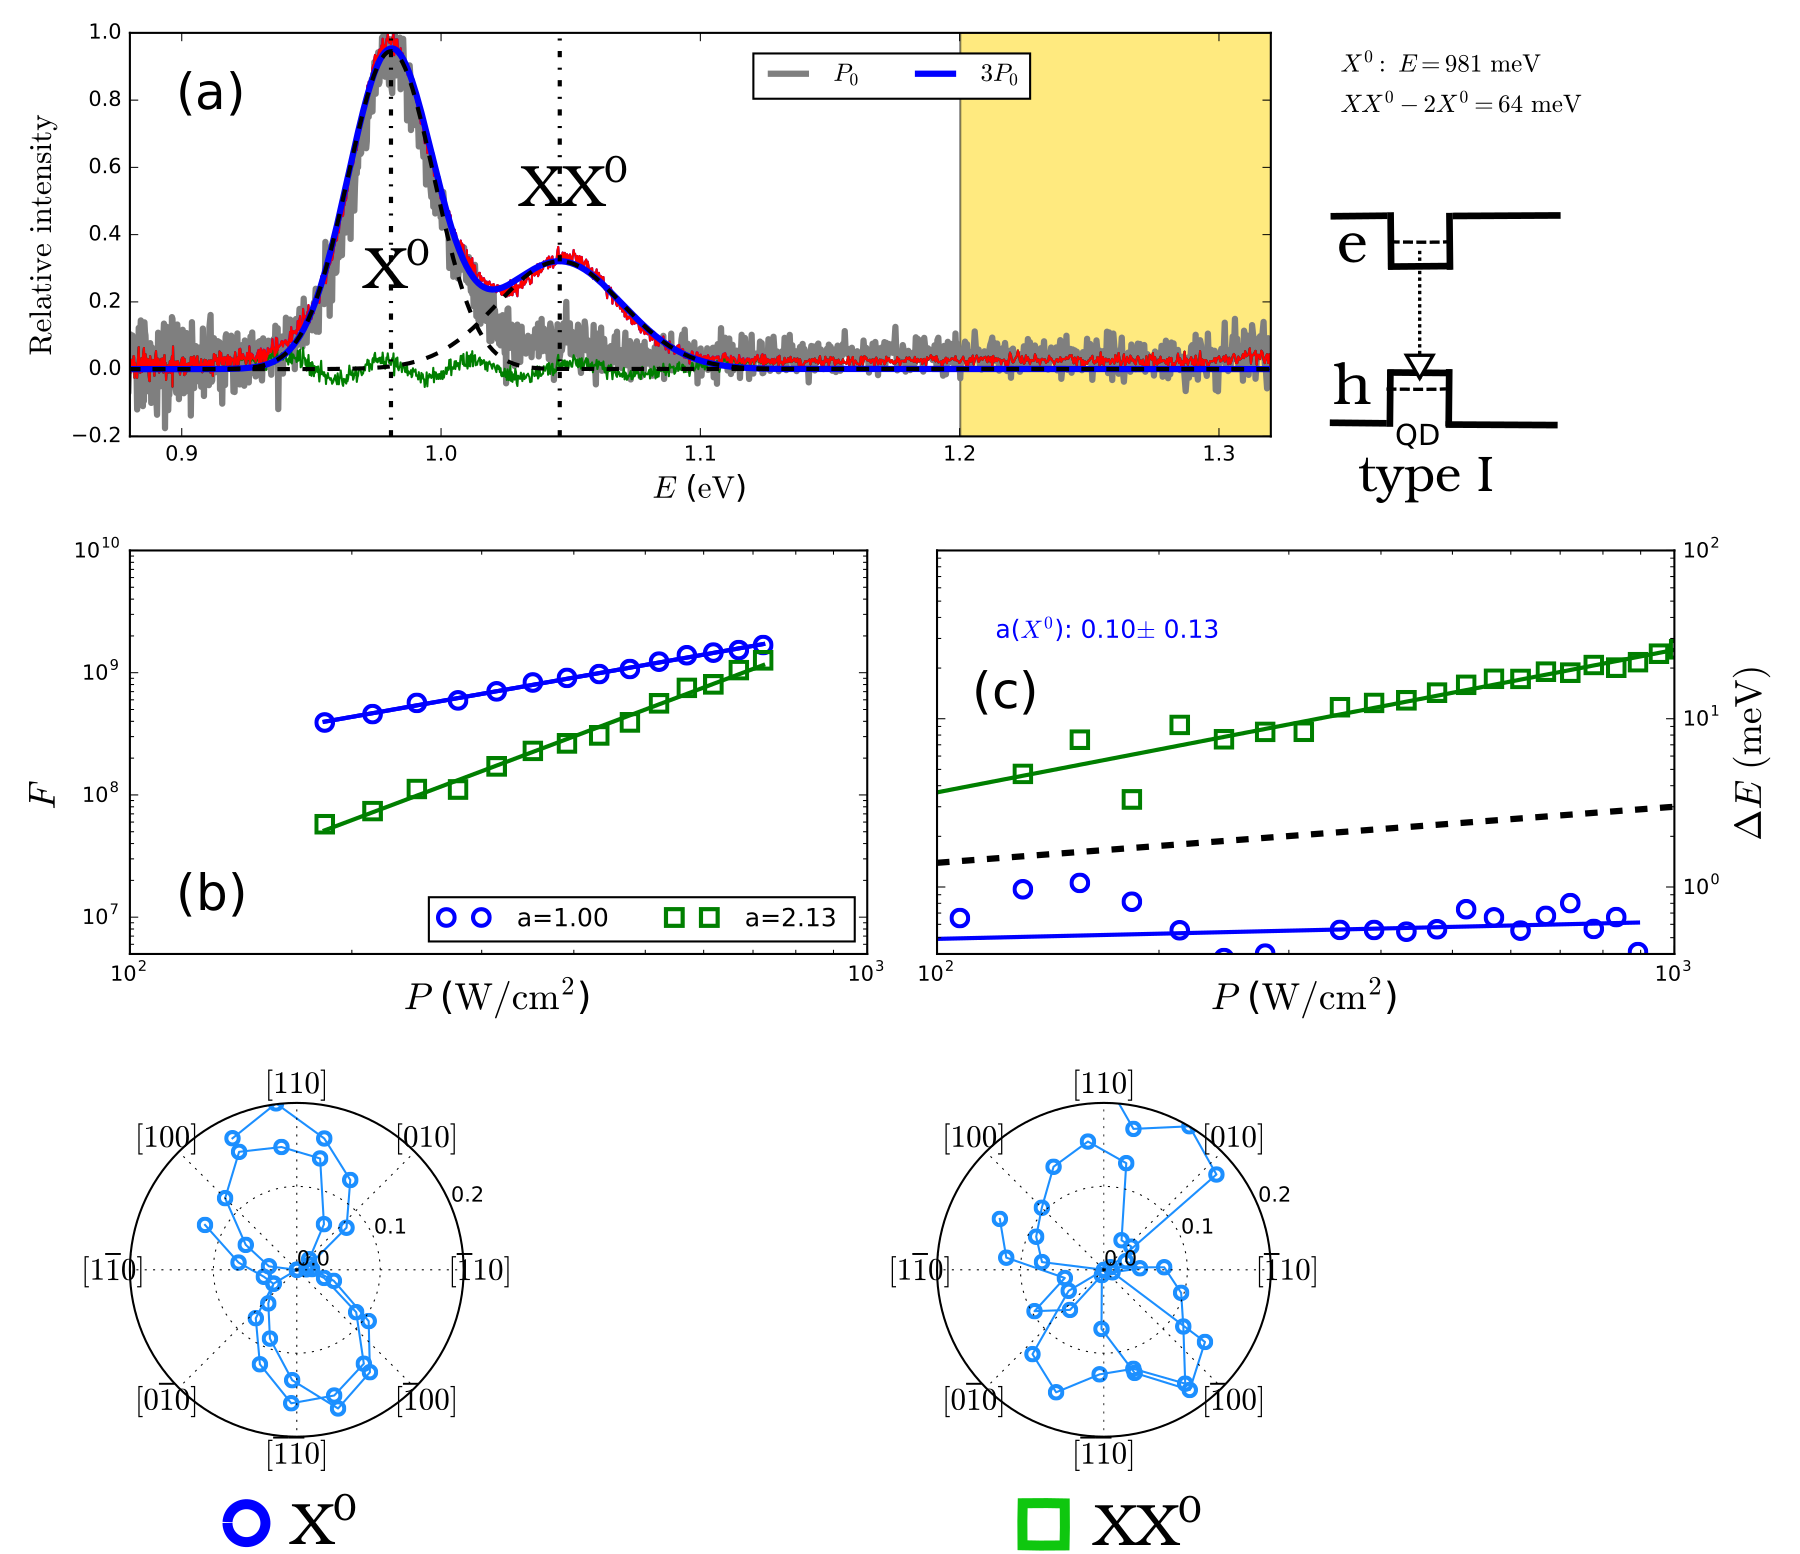
\includegraphics[width=0.9\linewidth]{/Sci_rep/article/671C}
	\caption{Results for type-I InAs/GaAs QDs. The outline of the figure is similar as in Fig.~\ref{fig:sci_rep_typeII}.}
	\label{fig:671C}
\end{figure}

In order to make our results more general we repeated the aforementioned measurements on 16~different QD samples. The results of those are given in the Appendix~\ref{chapter:appendix_SciRep} in Figs.~\ref{fig:sup:osc_slope} for the exponent in $F\propto P^a$, Fig.~\ref{fig:sup:mean_blueshift} for the mean emission energy shift, Fig.~\ref{fig:sup:mean_a_blueshift} for the mean $a$ in $\Delta E \propto P^a$, and Fig.~\ref{fig:sup:pol} for $\alpha_{\mathrm{max}}$, and $C_{\mathrm{max}}$, respectively.
\newpage 





\section{Model of blue-shift}\label{sec:scirep_pumpingmodel}
In PL experiments the blue-shift of the emission energy $\Delta E$ with increasing $P$ in type-II confined QDs is usually observed, however, the physical nature of this phenomenon is still discussed. Currently, two competing hypotheses are put forward in this respect.

The \textbf{state-filling} model stemming from the observation of large radiative lifetime of the emission from type-II QDs~\citep{Liao2009,Nishikawa2012,Sato2012,Pavarelli2012,Young2014}. In this model, the blue-shift is caused by a larger proportion of the radiative transitions between electronic levels higher in energy than the ground state if the pumping rate exceeds the emission rate of the ground state transition which is often the case for type-II QDs~\citep{Gradkowski2012}. In addition to this energetic aspect, the spatial localization of the wave functions associated with the states involved in the state-filling induces a capacitive charging effect~\citep{Muller-Kirsch2001}, also contributing to the overall blue-shift of the emission.


The second hypothesis dubbed \textbf{band-bending} explains blue-shift as a change of the confinement potential for holes close to the QD~\citep{LiuSteer,Jin,Hatami1998,Jo2012}. In the specific framework of infinite triangular quantum wells, it was speculated that this mechanism induces a $\Delta E \propto P^{1/3}$ dependence~\cite{Ledentsov1995,Kuokstis2002,Jo2012}. While the validity of this power law for different systems is arguable, it was often used in the literature for discussing the properties of GaSb/GaAs QDs~\cite{HATAMI1995,Hatami1998}.

Our experimental results presented in Figs.~\ref{fig:sci_rep_typeII} and \ref{fig:scirep_typeIq} are not consistent with the power law usually associated with band-bending, and require a specific interpretation. Therefore, we follow an approach similar to that of Gradkowski\textit{~et~al}., see Ref.~\citep{Gradkowski2012}. Because electronic states in QDs are multi-particle in nature, we employed so-called semi-self-consistent CI (SSCCI) approach developed by the supervisor to characterize the energy shift with $P$.

We now proceed with overview of SSCCI method. Firstly, a certain concentration of background electrons $c_e$ in QD body and holes $c_h$ in CL were defined, reflecting the spatially indirect nature of charges in the type-II system, to produce a background electric potential in QD and CL. Because we investigate system in a steady-state pumping regime, $c_h-c_e=0$. In other parts of the simulation space (GaAs matrix) we set $c_h=c_e=0$. Then, the single particle Schrödinger and Poisson equations for the system with these background potentials are solved self-consistently with all diagonal matrix elements of $J_{eh}$ resulting from the CI calculation set to zero since we assume those to be already included in the single-particle energies obtained from the preceding self-consistent cycle.

The correspondence of concentration used in simulations with the experiment with the values of $P$ is obtained by~\cite{Kuokstis2002}
%
\begin{equation}
\label{eq:conc_to_P_recalc}
P=\frac{10^6\gamma E_{l}}{\alpha}c_q^2,
\end{equation}
where $c_q=c_e=c_h$ is the number of electron-hole pairs generated by a laser light with the emission energy $E_l$ (in our case 1.58~eV), $\alpha$ is the absorption coefficient of the sample material ($2.0\times 10^4$~cm$^{-1}$ for GaAs~\cite{landoltbornstein}), and $\gamma$ is the radiative recombination coefficient ($7.0\times 10^{-10}$~cm$^3$s$^{-1}$ in the case of GaAs~\cite{landoltbornstein}).

The results of the blue-shift of multi-excitonic energies with $P$ calculated by SSCCI are presented in Fig.~\ref{fig:scirep_pumpmodel} for CL thicknesses of 3~and~8~nm. Our model correctly predicts the ``bending" of $\Delta E$ in panels~(c) of Figs.~\ref{fig:sci_rep_typeII} and \ref{fig:scirep_typeIq}, and the presence of different slopes in the log-log graphs [indicated by marks 1 and 2 in Fig.~\ref{fig:scirep_pumpmodel}~(a)].  The fitted exponents (slopes in log-log graphs) are $a_1=0.87\pm0.02$ and $a_2=0.07\pm0.02$ for $d=$3~nm, and $a_1=0.54\pm0.02$ for 8~nm, respectively. For type II the exponent in sector 1 decreases while that in sector 2 increases with increasing $d$, up to an approximate $\Delta E\sim P^{1/3}$ dependence reached for thick CLs. The blue-shift is accompanied by a change of the spatial distribution of the hole wavefunction~\cite{Gradkowski2012}, see insets of Fig.~\ref{fig:scirep_pumpmodel}~(b): holes are ``squeezed" towards the QD body and, thus, towards the electrons~\cite{Gradkowski2012,Llorens2015}. 
%
\begin{figure}
	\centering
	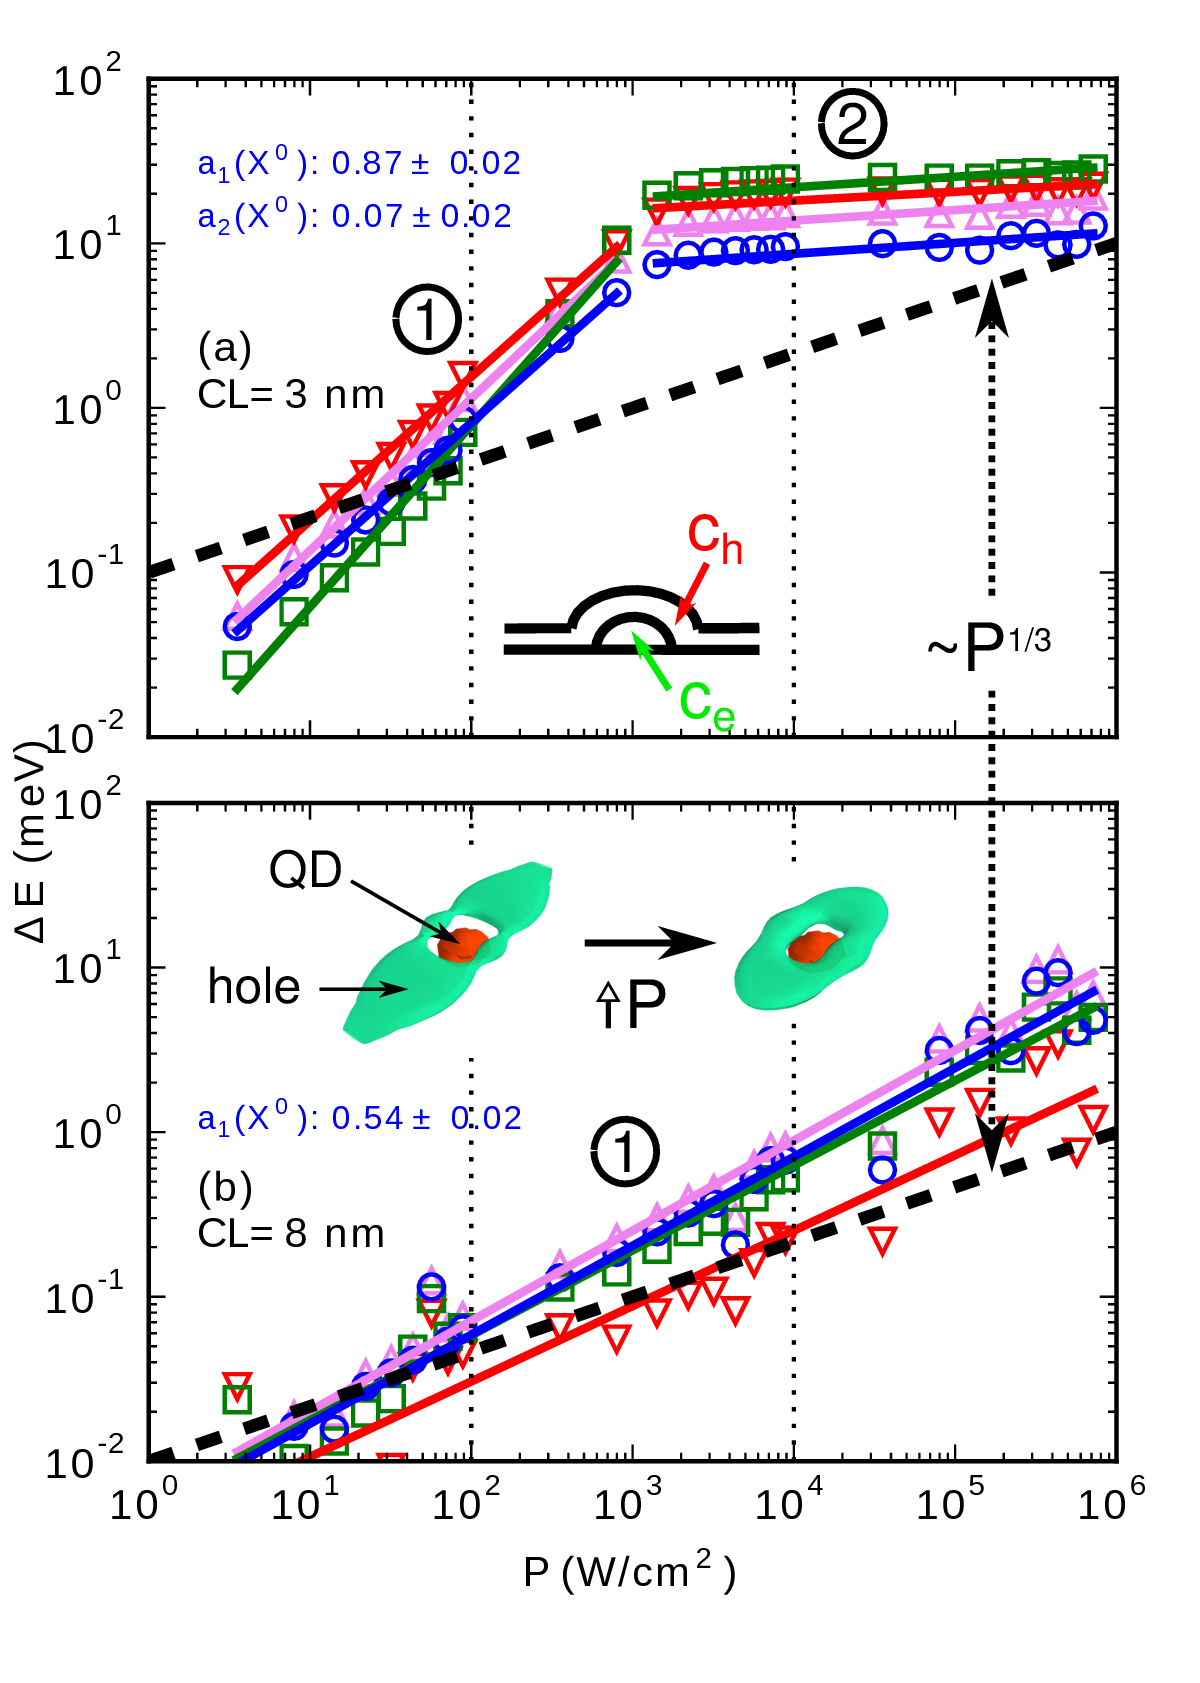
\includegraphics[width=0.68\linewidth]{/Sci_rep/article/pump_model}
	\caption{Energy shift $\Delta E$ as a function of $P$ for CL thickness $d$ of (a) 3~nm and (b) 8~nm for $X^0$ (blue circles), $X^+$ (magenta upward triangles), $X^-$ (red downward triangles), and $XX^0$ (green squares). The inset in (a) shows the background electron ($c_e$) concentration in QD and hole ($c_h$) in CL. The inset in (b) gives the hole probability density of 50~\% (green isosurfaces) for $d=8$~nm and two values of $P$; the dot is marked as a red lens in the middle of the hole wavefunction. The numbers 1 and 2 mark different segments of the dependency similarly to Figs.~\ref{fig:sci_rep_typeII} and \ref{fig:scirep_typeIq}. The fitted exponents $a_1$ and $a_2$ of $X^0$ are given in the insets of both panels. The dotted vertical lines in both panels roughly border the intervals where we have obtained in the measurements in Figs.~\ref{fig:sci_rep_typeII}  and~\ref{fig:scirep_typeIq}.}
	\label{fig:scirep_pumpmodel}
\end{figure}

The difference in $a_1$ between thinner and thicker CL can be qualitatively understood by inspecting the change in the lateral electron-hole dipole moment $p_{xy}$ with $P$. The total lateral potential for holes in type-II QDs might be written as $V_{xy}^\mathrm{total}=V_{xy}^\mathrm{bulk}-V^{\mathrm{piez}}_{xy}$, where $V^{\mathrm{bulk}}_{xy}$ is the energy of the holes in the bulk semiconductor. With increasing $P$ the hole wavefunction is shifted towards that of the electrons, thus $V^{\mathrm{piez}}_{xy}$ is reduced, so that both $V^{\mathrm{total}}_{xy}$ and the single-particle transition energies increase. Because $p_{xy}$ is larger in the QDs with thin CL than in those with a thick CL, we can infer that the rate of blue-shift of single-particle transition energies with $P$ should be larger for QDs with thinner CLs.

The meaning of $c_e$ and $c_h$ in our calculations is that of an average occupation of charge traps~\cite{Reimer2016} in QD and CL, respectively, thus, there is probably an important contribution of trap-state filing effect. 

Finally, our model of blue-shift is more consistent with the ``band-bending'' hypothesis presented above if the changes of the confinement potential of quasiparticles are due to filling of charge traps.

\section*{Conclusions}
We have experimentally studied the excitonic structure of type-II InAs/GaAsSb/GaAs quantum dots by intensity and polarization resolved photoluminescence spectroscopy. Based on intensity resolved photoluminescence we identify multiparticle optical transitions of neutral exciton, biexciton, and negative trion, respectively. Our identification is supported by full configuration interaction calculations where the similar binding energies of these complexes have been predicted. 

The polarization-resolved photoluminescence allows us to distinguish optical transitions originating from quantum dots, where emission anisotropy of the complexes is oriented along [110]~crystallographic direction, from the transition between interface bulk GaAs-GaAsSb capping layer states and quantum dots having perpendicular orientation of polarization.

The blue-shift of emission energy with increasing excitation laser power is observed for InAs/GaAsSb/GaAs quantum dot samples. This blue-shift is simulated by semi-self-consistent configuration interaction method with added background potential in quantum dot area.

The blue-shift model for thicker capping layer gives similar behaviour as usually used $\Delta E\propto P^{1/3}$ approximation, for thin capping layer, a stronger blue-shift is predicted up to a critical excitation power followed by slighter increase for thick layer. This two segment behaviour is experimentally observed.
\newpage